\documentclass[a4paper, 10pt, final, garamond]{book}
\usepackage{cours-preambule}

\makeatletter
\renewcommand{\@chapapp}{Thermodynamique -- chapitre}
\makeatother

\hfuzz=5.002pt

% \toggletrue{student}
% \toggletrue{corrige}
% \renewcommand{\mycol}{black}
% \renewcommand{\mycol}{gray}

\begin{document}
\setcounter{chapter}{1}

% \settype{enon}
% \settype{solu_prof}
% \settype{solu_stud}

\chapter{\cswitch{Correction du TD}{TD~: Échanges d'énergie des systèmes
	  thermodynamiques}}

\resetQ
\section{Transformations de tous les jours}
\enonce{%
	Caractérisez les transformations thermodynamiques suivantes~:
}%

\QR{%
	Vous placez dans un thermos du thé bouillant et de l'eau froide.
}{%
	Transformation adiabatique d'une phase condensée, isobare et isochore.
}%
\QR{%
	Vous oubliez votre tasse de café dans la cuisine la journée.
}{%
	Transformation monotherme, isobare et isochore.
}%

\resetQ
\section{Travail reçu le long d'un chemin donné}
\enonce{%
	Un système constitué de $n$ moles de gaz parfait subit une transformation d'un
	état initial A $(P_1 = \SI{4.0}{bar}, V_1 = \SI{10}{L}, T_1 = \SI{600}{K})$
	vers un état final B $(P_2 = \SI{1.0}{bar}, V_2 = \SI{20}{L}, T_2)$.
}%
\QR{%
	Déterminer $T_2$.
}{%
	\leavevmode\vspace*{-15pt}\relax
	\begin{gather*}
		\beforetext{Le gaz étant parfait,}
		P_1V_1 = nRT_1
		\qet
		P_2V_2 = nRT_2
		\\\Lra
		n = \frac{P_1V_1}{RT_1}
		\qet
		\boxed{T_2 = \frac{P_2V_2}{P_1V_1}T_1}
		\\\Ra
		\xul{T_2 = \SI{300}{K}}
	\end{gather*}
}%
\QR{%
	Cette transformation est constituée de deux étapes~: une transformation
	isobare de A vers C puis une transformation isochore de C vers B. Déterminer
	le travail $W\ind{AB}$.
}{%
	$W\ind{AB} = W\ind{AC} + W\ind{CB}$.
	\begin{itemize}
		\item $W\ind{CB} = 0$ car isochore~;
		\item
		      \begin{gather*}
			      \beforetext{Si $A \ra C$ quasi-statique,}
			      W\ind{AC} = - \int_{A}^{C} P \dd{V}
			      \\\beforetext{Comme $A \ra C$ isobare, $P = P_1$ et}
			      W\ind{AC} = -P_1 (V_2-V_1)
		      \end{gather*}
	\end{itemize}
	Ainsi,
	\[
		W\ind{AB} = W\ind{AC}
		\Ra
		\xul{W\ind{AB} = \SI{-4.0}{kJ}}
	\]
}%
\QR{%
	On considère un autre chemin~: une transformation isochore de A vers D puis
	une transformation isobare de D vers B. Déterminer le travail $W\ind{AB}$.
}{%
	De même que précédemment, la transformation isochore a un travail nul, donc
	seule la transformation de D vers B travaille, et $W\ind{AB} = W\ind{DB}$.
	Seulement, la pression de l'isobare n'est plus la même, et on trouve
	\[
		W\ind{AB} = W\ind{DB} = -P_2 (V_2-V_1)
		\\\Ra
		\xul{W\ind{AB} = \SI{-1.0}{kJ}}
	\]
}%
\QR{%
	Représenter ces deux transformations sur un schéma et retrouver graphiquement
	quelle transformation a le plus grand travail et le signe dudit travail.
}{%
	% TODO: Graphique rM, inkscape~?
}%

\resetQ
\section{Diagramme de \textsc{Clapeyron}}
\enonce{%
	Considérons un système fermé qui subit une transformation d'un état
	d'équilibre initial $(P_i, V_i)$ à un état d'équilibre final $(P_f, V_f)$, de
	manière mécaniquement réversible.
}%
\QR{%
	Représenter les différentes transformations dans un diagramme de
	\textsc{Clapeyron} $(P,v)$~: isochore, isobare, isotherme d'un gaz parfait,
	adiabatique d'un gaz parfait, caractérisée par $PV^{\gamma} = \cte$
	avec $\gamma > 1$.
}{%
	% TODO: Pareil
}%
\QR{%
	Faire le lien entre l'aire sous la courbe et le travail des forces de
	pression dans ce diagramme.
}{%
	\leavevmode\vspace*{-15pt}\relax
	\begin{gather*}
		\Ac =
		\int_{v_i}^{v_f} P \dd{v} =
		-\frac{1}{m} \left( - \int_{V_i}^{V_f} P \dd{V} \right)
		\\\beforetext{Or $P = P\ind{ext}$ pour quasi-statique}
		\boxed{\Ac = - \frac{W_p}{m}}
	\end{gather*}
}%
\QR{%
	Pour une transformation cyclique, faire le lien entre le sens de parcours du
	cycle et le signe du travail au cours d'un cycle.
}{%
	$\dd{V} > 0 \Lra W_p < 0$ et inversement. Or, si le cycle est parcouru dans le
	\textbf{sens direct}, alors la transformation de $\dd{V} > 0$ passe en-dessous
	de la transformation de $\dd{V} < 0$~; ainsi l'aire entourée correspond à un
	travail \textbf{positif}.
}%

\resetQ
\section{Calculs de travaux et transferts thermiques}
\enonce{%
On considère trois moles de dioxygène, gaz supposé parfait, qu'on peut faire
passer de l'état initial A $(P_A, V_A, T_A)$ à l'état final B $(P_B, V_B,
	T_B)$ par trois transformations distinctes~:
\begin{itemize}
	\item A1B isotherme~;
	\item A2B représentée par une droite dans le diagramme $(P,V)$~;
	\item A3B composée d'une transformation à volume constant, suivie d'une
	      transformation à pression constante.
\end{itemize}
On considère l'équilibre thermodynamique interne conservé à tout instant. On
donne $P_B = 3 P_A$, $T_A = \SI{300}{K}$ et $R =
	\SI{8.314}{J.K^{-1}.mol^{-1}}$.
}%
\QR{%
	Représenter les trois transformations dans le diagramme $(P,V)$.
}{%
	% TODO: à faire
}%
\QR{%
	Déterminer la température $T_B$ et le volume $V_B$
}{%
	solu
}%
\QR{%
	Calculer les travaux reçus par le système pour ces trois transformations.
	Commentez.
}{%
	solu
}%
\QR{%
	Calculer les transferts thermiques reçus par le système pour ces trois
	transformations. On donne le premier principe de la thermodynamique~:
	$\Delta{U} = W + Q$.
}{%
	solu
}%

\resetQ
\section{Étude d'un compresseur}
\enonce{%
	\noindent
	\begin{minipage}[c]{.48\linewidth}
		On s'intéresse au compresseur d'un moteur à air comprimé, comme celui d'un
		marteau-piqueur par exemple. L'air est assimilé à un gaz parfait. Il est
		aspiré dans les conditions atmosphériques, sous la pression $P_0 =
			\SI{1}{bar}$ et à la température $T_0 = \SI{290}{K}$, jusqu'au volume $V_m$.
		Il est ensuite comprimé jusqu'à la pression $P_1$ où il occupe un volume
		$V_1$, et est refoulé à la température $T_1$ dans un milieu où la pression est
		$P_1 = \SI{6}{bar}$.
	\end{minipage}
	\hfill
	\begin{minipage}[c]{.48\linewidth}
		\begin{center}
			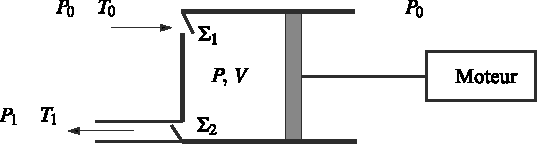
\includegraphics[width=\linewidth]{compresseur-plain}
		\end{center}
	\end{minipage}
	Bien que le mécanisme réel d'un compresseur soit
	différent, on suppose que celui-ci fonctionne comme une pompe à piston, qui se
	compose d'un cylindre, d'un piston coulissant entraîné par un moteur et de
	deux soupapes~:
	\begin{itemize}
		\item La soupape d'entrée $\Sigma_1$ est ouverte si la pression $P$ dans le
		      corps de la pompe est inférieure ou égale à la pression atmosphérique
		      $P_0$~;
		\item La soupape de sortie $\Sigma_2$ est ouverte si $P$ est supérieure à
		      $P_1$~;
		\item Le volume $V$ du corps de pompe est compris entre $0$ et $V_m$~;
		\item À chaque cycle (un aller-retour du piston), la pompe aspire et refoule
		      une mole d'air.
	\end{itemize}
}%
\begin{blocQR}
	\item
	\QR{%
		Tracer sur un diagramme de \textsc{Watt} $(P,V)$ l'allure de la courbe
		représentant un aller-retour du piston. Indiquer le sens de parcous par une
		flèche.
	}{%
		solu
	}%
	\QR{%
		Montrer que le travail de l'air situé à droite du piston est nul sur un
		aller-retour.
	}{%
		solu
	}%
	\QR{%
		Montrer que le travail fourni par le moteur qui actionne le piston est égal à
		l'aire d'une surface sur le diagramme. On supposera que le mouvement est assez
		lent pour que l'évolution soit mécaniquement réversible.
	}{%
		solu
	}%
\end{blocQR}
\QR{%
	Pendent la phase de compression, l'air suit une loi polytropique $PV^k =
		\cte$. Il sort du compresseur à la température $T_1 = \SI{391}{K}$. Trouver la
	valeur de $k$.
}{%
	solu
}%
\QR{%
	Exprimer le travail mécanique $W\ind{moteur}$ fourni par le moteur pendant un
	aller-retour en fonction de $n, R, k, T_1$ et $T_0$.
}{%
	solu
}%
\QR{%
	Le débit massique de l'air dans le compresseur est $D_m =
		\SI{0.013}{kg.s^{-1}}$. Calculer la puissance $\Pc\ind{moteur}$ fournie par le
	moteur.
}{%
	solu
}%

\resetQ
\section{Apport d'énergie électrique}
\enonce{%
	Un récipient de volume $2V_0 = \SI{4.0}{L}$ est partagé en deux compartiments
	(1) et (2), séparés par une paroi mobile et athermane. Le premier compartiment
	est calorifugé, le second est entouré de parois diathermes. Chacun contient
	$n$ moles d'un gaz parfait diatomique, qui occupe un volume initial $V_0$ sous
	la pression $P_0 = \SI{1.0}{bar}$ et la température $T_0 = \SI{300}{K}$,
	température de l'air extérieur.
	\bigbreak
	Dans le compartiment (1) se trouve une résistance électrique $R$, dans
	laquelle on fait passer un courant $I$. Le phénomène, assez lent, conduit au
	bout d'un temps $\tau$ à obtenir une pression dans le compartiment (1) telle
	que $P_1 = 2P_0$.
}%
\QR{%
	Déterminer et calculer les grandeurs $P_2$, $V_2$ et $T_2$ au bout du temps
	$\tau$ dans le compartiment.
}{%
	solu
}%
\QR{%
	En déduire les expressions et les valeurs de $V_1$ et de $T_1$.
}{%
	solu
}%
\QR{%
	Déterminer et calculer les variations d'énergie interne $\Delta{U_1}$ et
	$\Delta{U_2}$.
}{%
	solu
}%
\QR{%
	Quel travail $W_{p,2}$ a été reçu par le compartiment (2)~? Combien vaut
	$W_{p,1}$ reçu par le compartiment (1)~?
}{%
	solu
}%
\QR{%
	Comment s'exprime l'énergie thermique reçue par le compartiment (1)~? La
	relier à $U$ et $W_{p,1}$ grâce au premier principe $\Delta{U} = W + Q$.
	Déterminer alors la valeur de $\tau$.
}{%
	solu
}%

\end{document}
